\documentclass[10pt, a4paper]{article}
\usepackage[utf8x]{inputenc}            % Acentos, ñ, etc.
\usepackage{graphicx}                   % Gráficos
\usepackage[spanish]{babel}             % Macros en español
\usepackage{caratula}                   % Carátula
\usepackage{geometry}                   % Márgenes
\begin{document}


Q

¿Cuál es el espacio de estados?
Cada configuracion posible del tablero es un estado, es decir guardamos para cada posición del tablero si hay una ficha y de que jugador. Muchos de esos estados son inalcanzables, ya que toda ficha debe estar inmediatamente por encima de otra ficha. Tampoco consideramos estados en los que hay cuatro fichas alineadas (ya sea de forma vertical, horizontal o diagonal). 
Cada accion se corresponde con insertar una ficha en alguna de las columnas. La ficha será asignada a la fila inmediatamente superior a la fila donde estaba la ficha más arriba en la misma columna.

Las recompensas a las acciones tomadas se otorgan después de que juegue el rival, excepto en los casos en los que la partida finaliza.

graficos posibles:
grafico de jugador entrenado (solamente la curva sin la del rival) variando los valores de epsilon fijos (y un mismo jugador que va variando)
idem gamma
alpha

variando las recompensas?

q(vsRandom) vs q(vsQ) con epsilon 0, osea no siguen aprendiendo.


4x4 y ver si eso lleva a  mas empates
comparar si cambiamos ganancia de empate a 0.
¿juagada ganadora? Veamos si siempre empieza el jugador 1.


cuán rápido se puede explorar?, ¿cómo cambia la inicialización de Q con respecto a la velocidad de aprendizaje?, ¿qué importancia tiene la temperatura y la velocidad con que se enfría el sistema si se decide usar la distribution Boltzmann?, ¿qué efecto tiene cambiar la tasa de aprendizaje?, etc.


¿Cuál es el espacio de estados?, ¿cuán rápido se puede explorar?, ¿cómo cambia la inicialización de Q con respecto a la velocidad de aprendizaje?, ¿qué importancia tiene la temperatura y la velocidad con que se enfría el sistema si se decide usar la distribution Boltzmann?, ¿qué efecto tiene cambiar la tasa de aprendizaje?, etc.

\newgeometry{left=1cm,right=1cm}


\begin{figure}[ht]
  \begin{minipage}[c]{1\textwidth}
	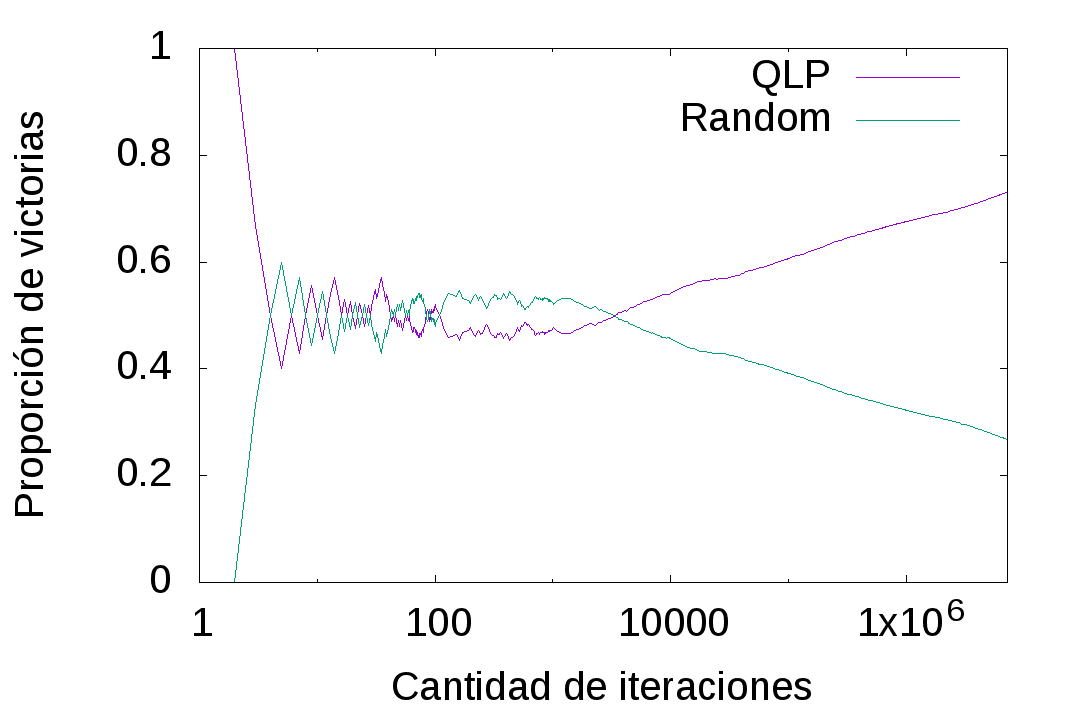
\includegraphics[scale=0.32]{Initial/QvR.png}
	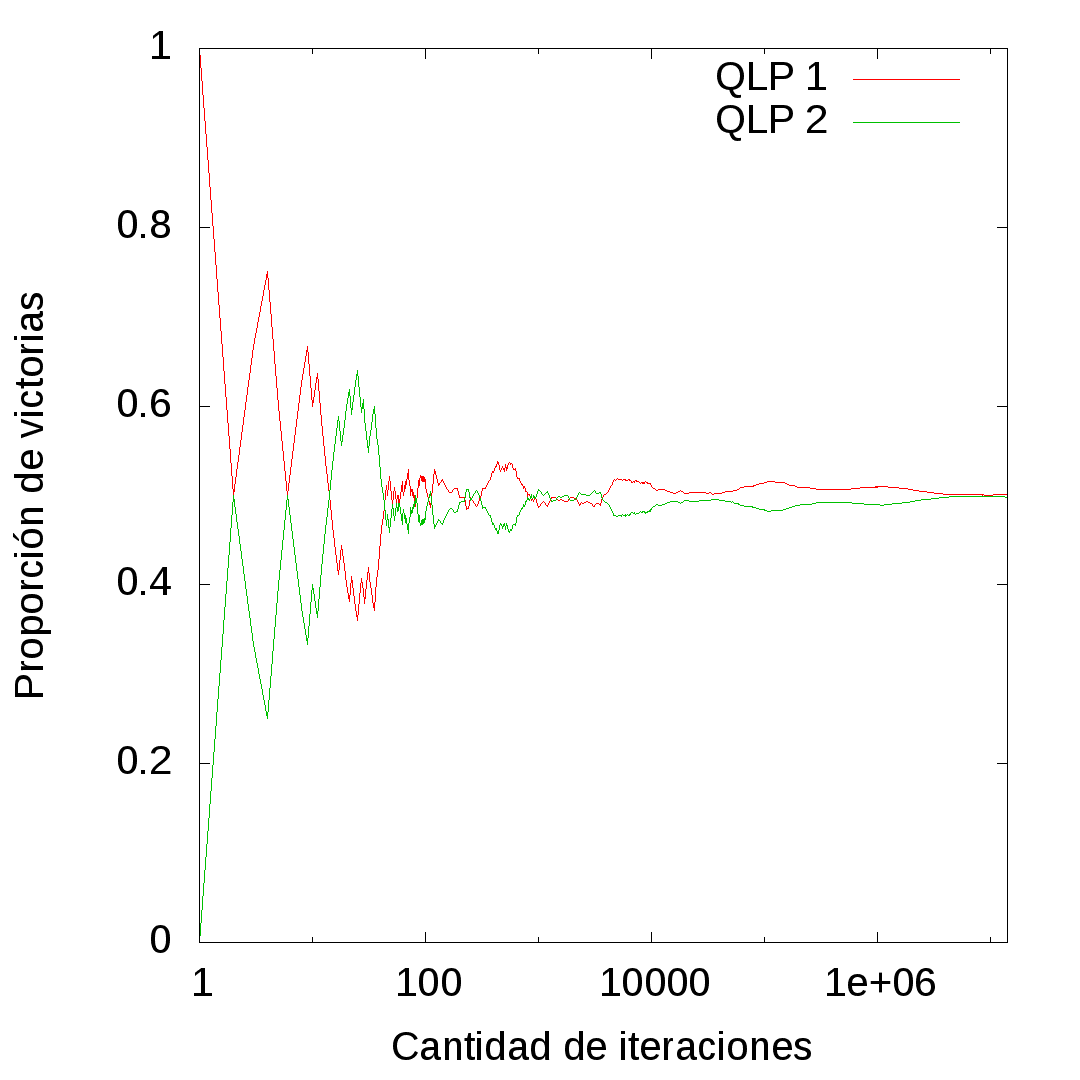
\includegraphics[scale=0.32]{Initial/QvQ.png}
  \end{minipage}
\end{figure}

\begin{figure}[ht]
 \centering
  \begin{minipage}[c]{1\textwidth}
	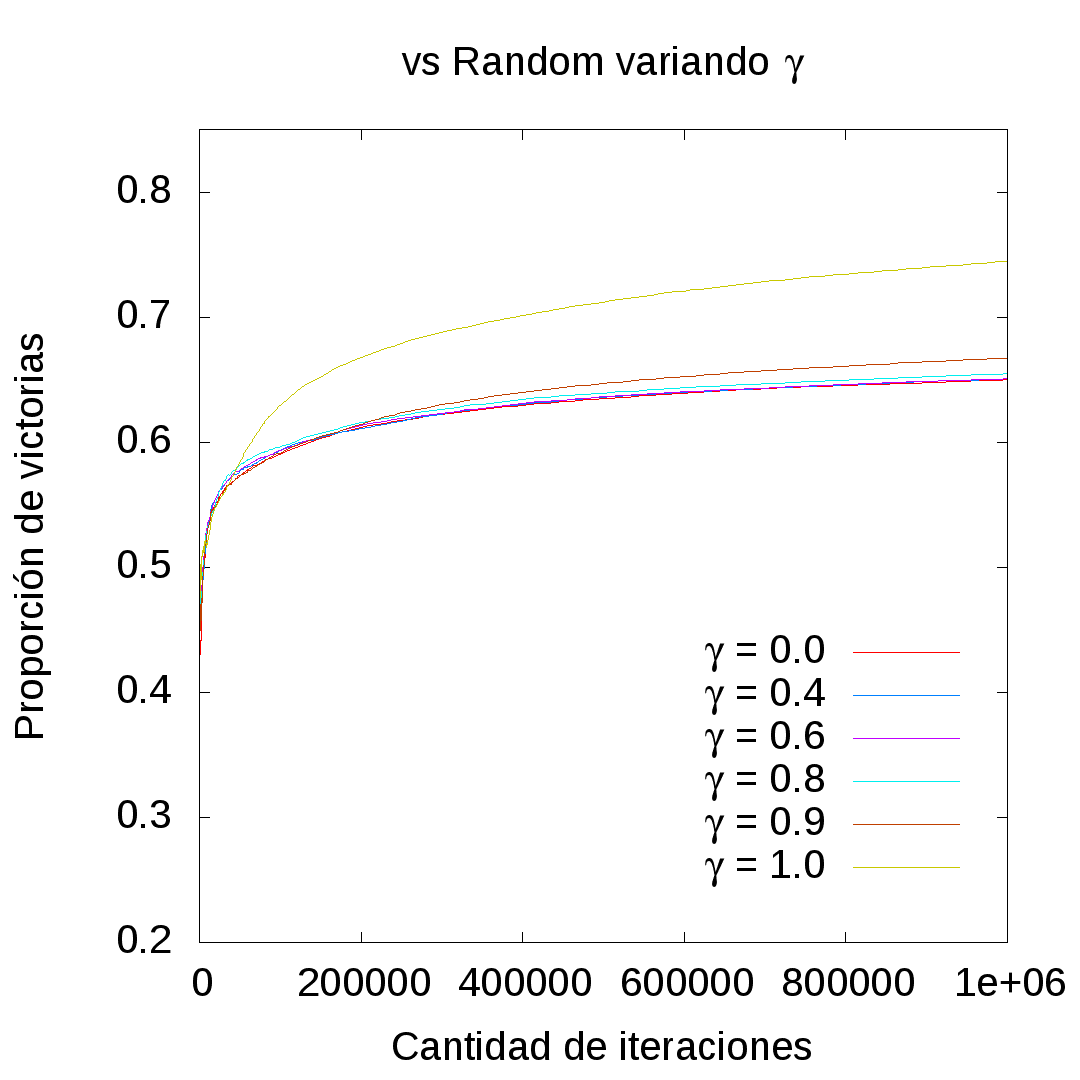
\includegraphics[scale=0.32]{GammaR.png}
	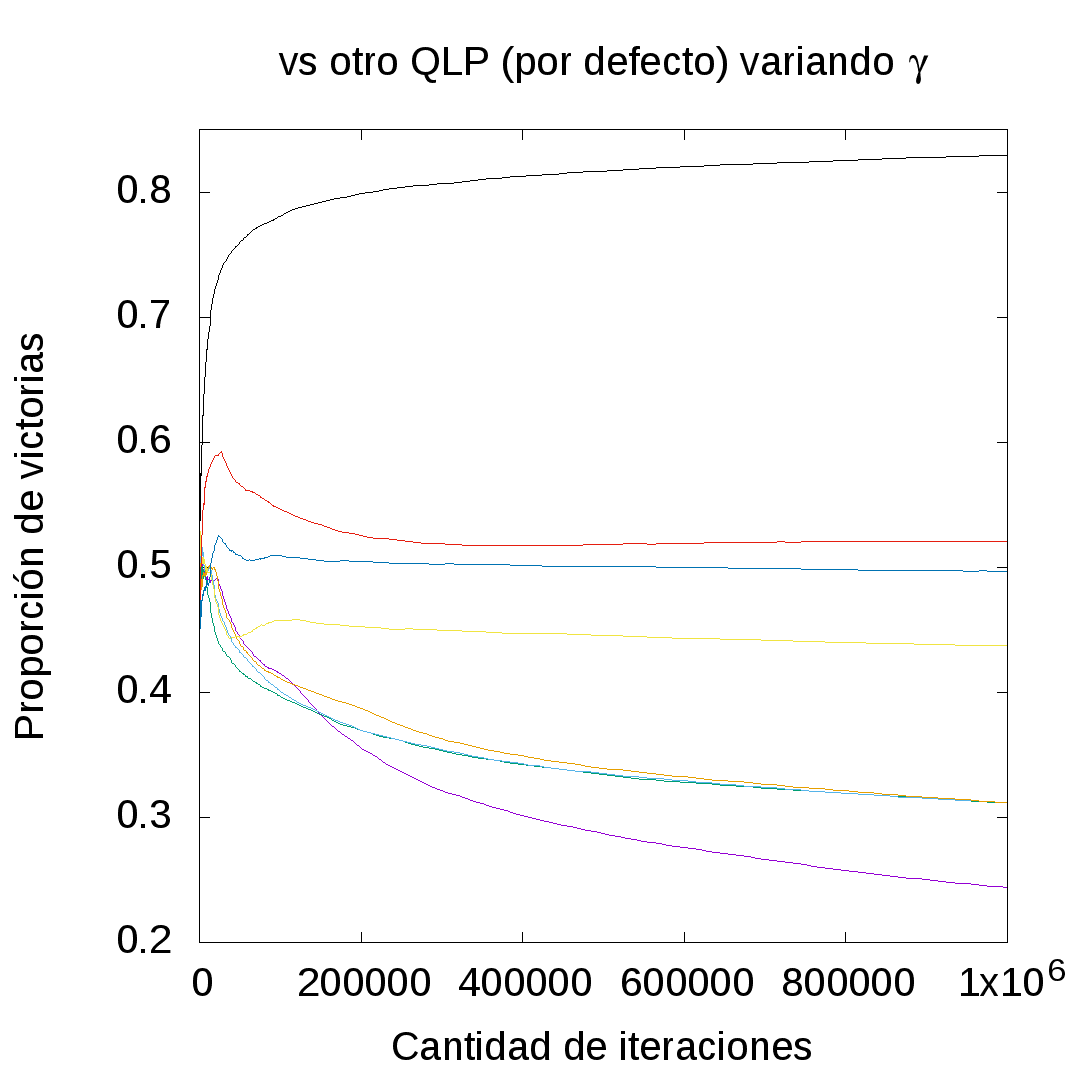
\includegraphics[scale=0.32]{GammaQ.png}
  \end{minipage}
\end{figure}
\begin{figure}[ht]
  \begin{minipage}[c]{1\textwidth}
	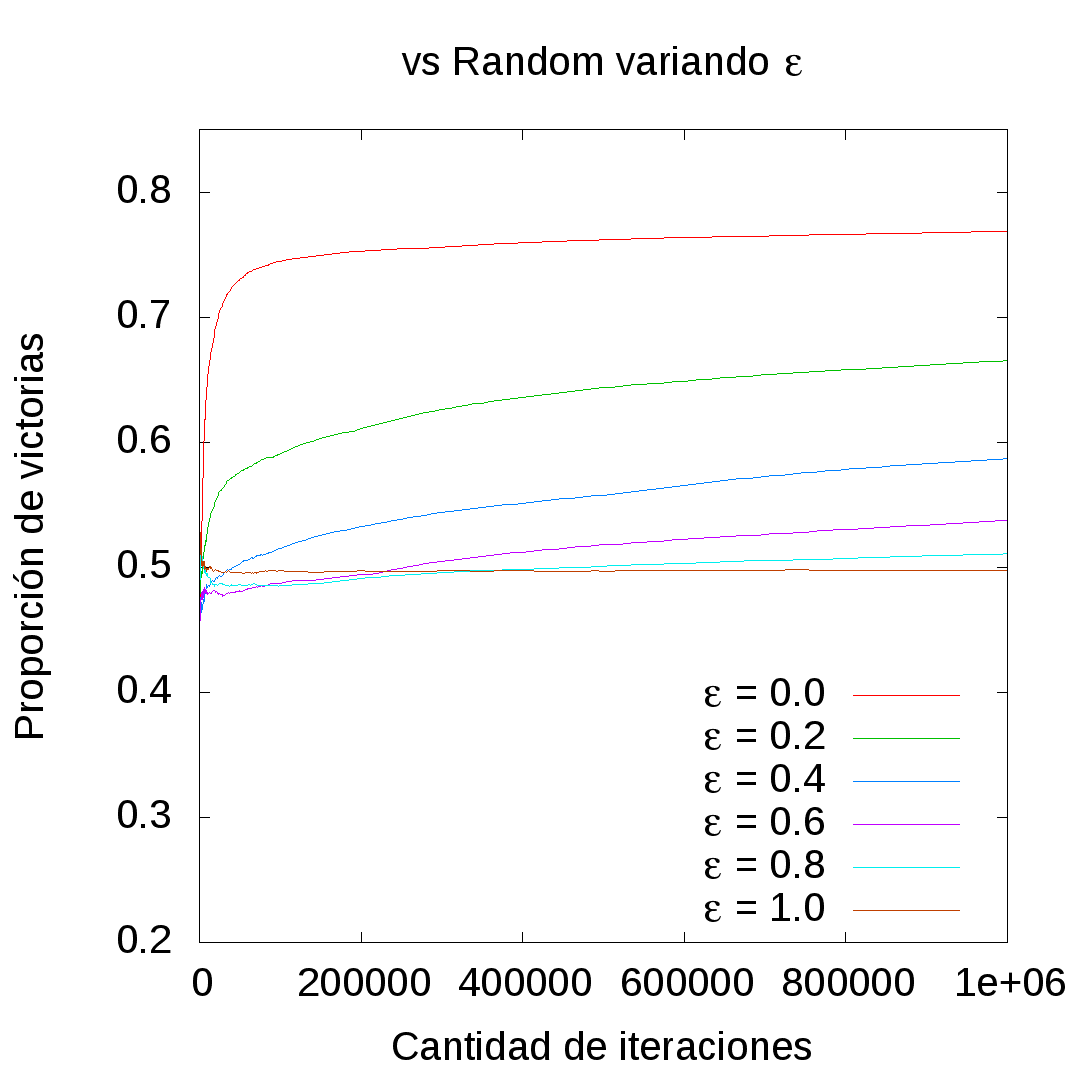
\includegraphics[scale=0.32]{EpsilonR.png}
	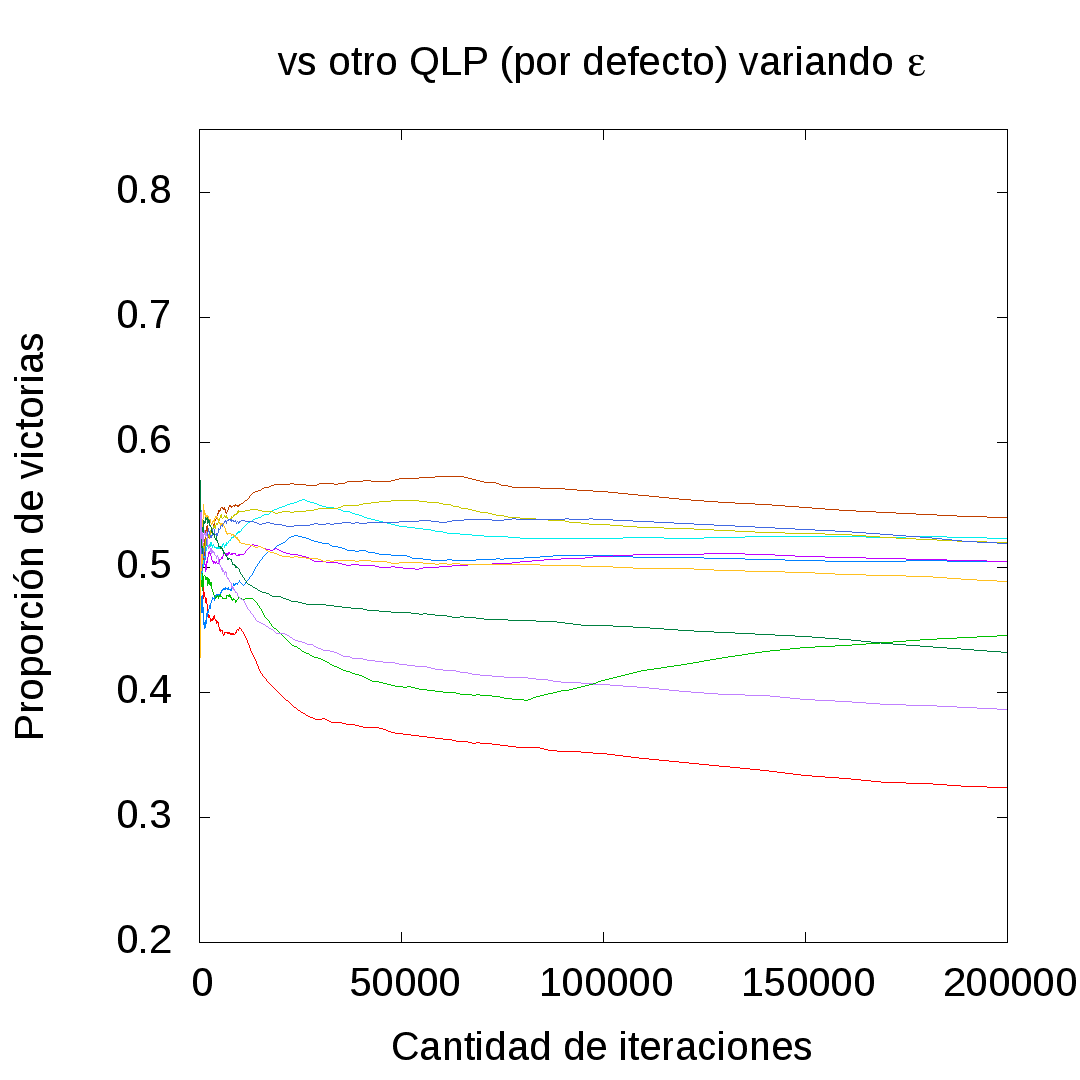
\includegraphics[scale=0.32]{EpsilonQ.png}
  \end{minipage}
\end{figure}
\begin{figure}[ht]
  \begin{minipage}[c]{1\textwidth}
	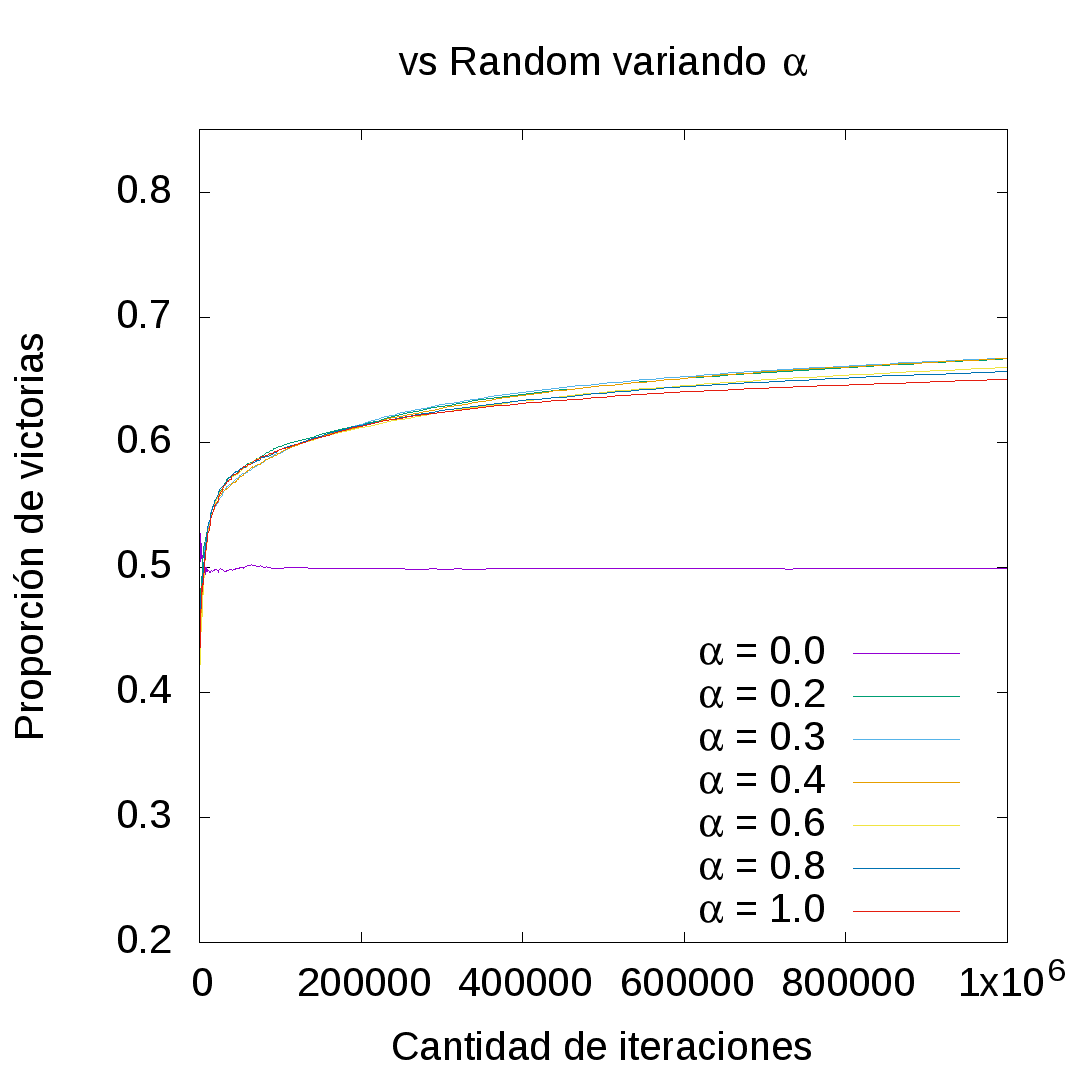
\includegraphics[scale=0.32]{AlphaR.png}
	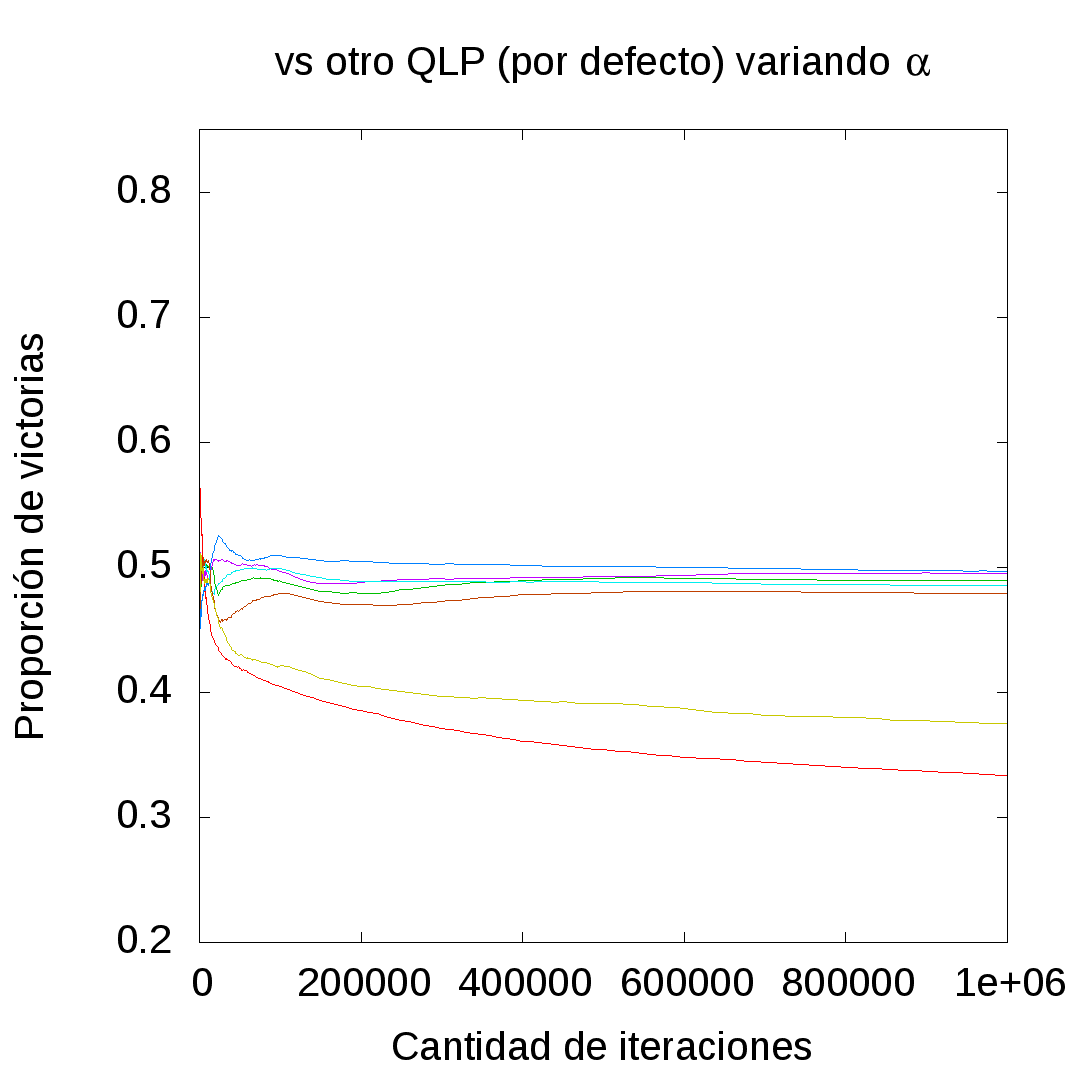
\includegraphics[scale=0.32]{AlphaQ.png}
	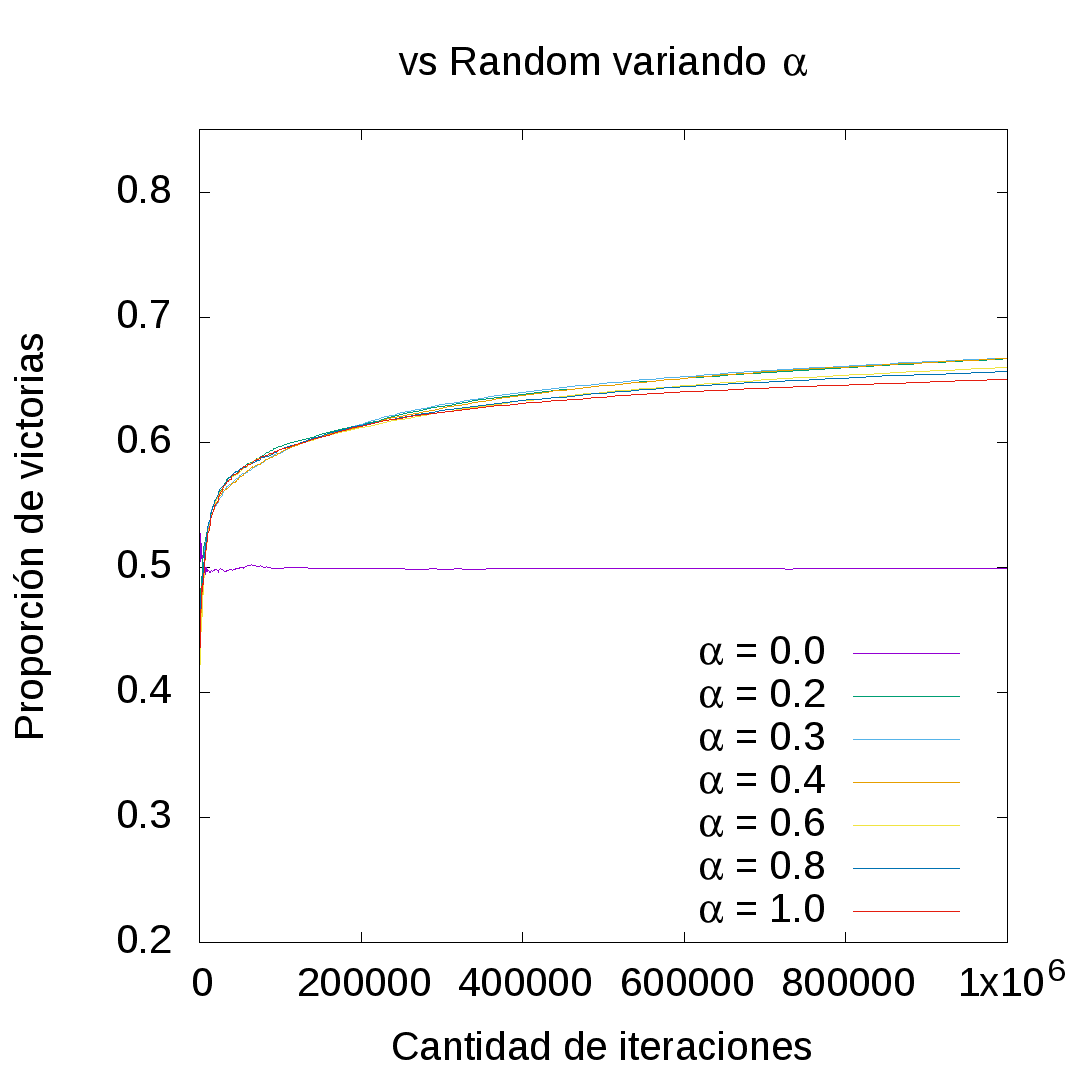
\includegraphics[trim=230mm 185mm 13mm 90mm, clip, scale=2.5]{AlphaR.png}
	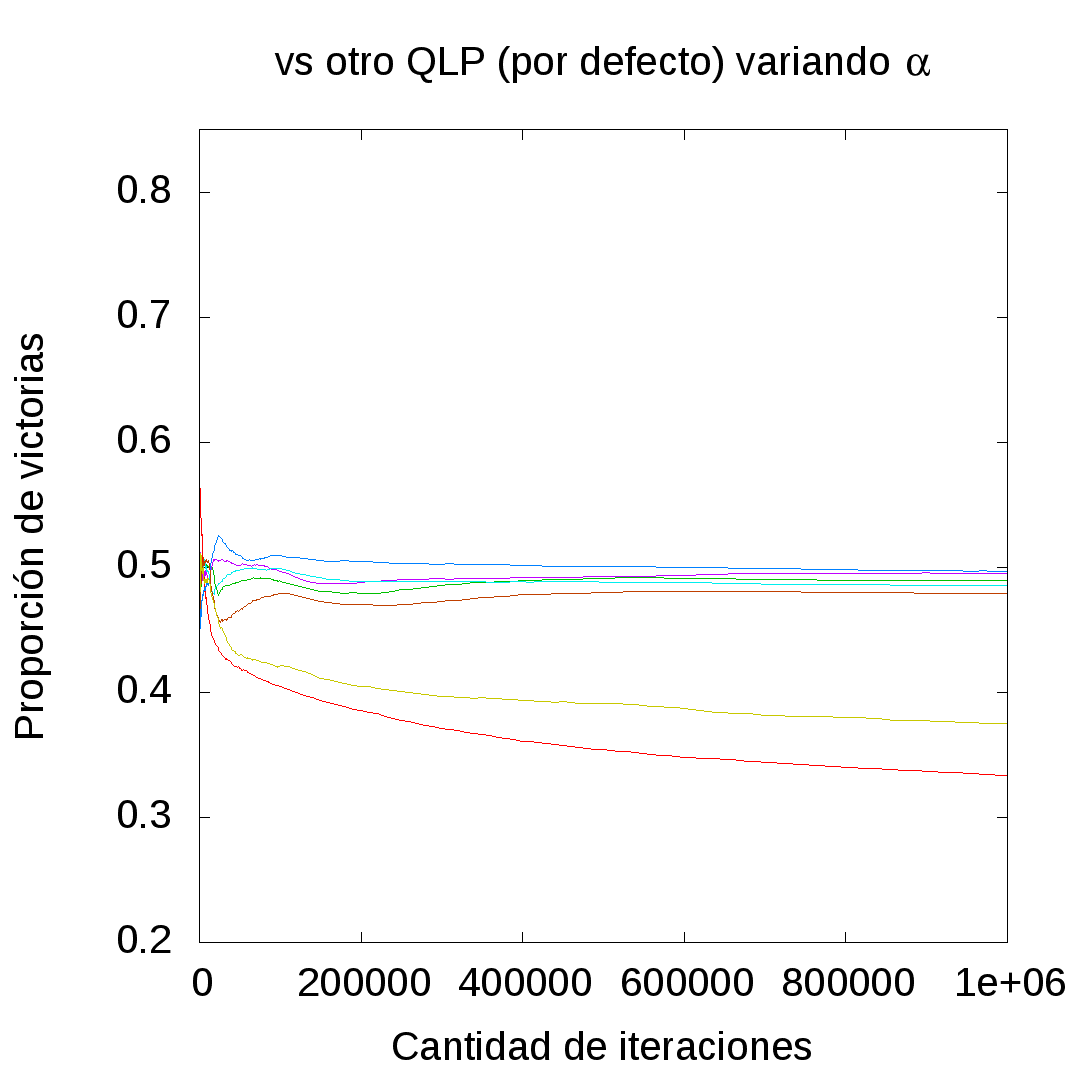
\includegraphics[trim=235mm 125mm 0mm 150mm, clip, scale=2.5]{AlphaQ.png}
  \end{minipage}
\end{figure}

\restoregeometry

Conclusiones: El jugador 1 aprendió la estrategia ganadora! Felicitaciones.

\end{document}
